\chapter{\difficult{Higher-dimensional Geometry}}\label{chapter:hdg}

    In this chapter we generalize certain constructions and theorems introduced in the previous chapters to the setting of higher categories. As such it can been as an analogue to Chapter \ref{chapter:hda} for (differential) geometry.

    The main references are \cite{higher_gauge, phd_schreiber}. For a refresher on (higher) category theory see chapter \ref{chapter:cat}. The section on smooth spaces is inspired by \cite{baez_convenient}. Section \ref{section:higher_lie_structures} gives a different approach to the higher-dimensional analogues of Lie algebras.

    ?? CITE BAEZ, SCHREIBER, BARTELS, ... ??

\section{Noncommutative geometry}\index{quantum!geometry}

    \newdef{Quantum metric}{\index{metric}
        Consider an FODC $(A,\Gamma)$ as in definition \ref{qa:fodc}. A generalized inner-product is a bimodule morphism $\langle\cdot|\cdot\rangle:\Gamma\otimes\Gamma\rightarrow A$. A (generalized) metric with respct to an inner product $\langle\cdot|\cdot\rangle$ is an element $g\in\Gamma\otimes\Gamma$ such that
        \begin{gather}
            \langle\omega|\cdot\rangle\otimes\mathbbm{1}(g) = \omega = \mathbbm{1}\otimes\langle\cdot|\omega\rangle(g)
        \end{gather}
        for all $\omega\in\Gamma$. This condition represents the invertibility of the metric.
    }

\section{Smooth spaces}\index{smooth!space}\label{section:smooth_spaces}

    In this section we consider some generalizations of spaces that are better behaved when considering their properties as a whole. Before moving to the smooth setting, we will first give a bit of history starting in the ordinary topological setting.

    The first problem in the study of the global properties of spaces arose in algebraic topology. When consider mapping spaces we sometimes like to use the currying operation \[C(X\times Y, Z)\rightarrow C(X, C(Y, Z)).\] However, in general, this is not a homeomorphism, i.e. currying does not define an adjunction and therefore $\mathbf{Top}$ is not Cartesian closed \ref{cat:closed}. This problem was treated by \textit{Steenrod} and others, and the solution was simply to restrict to a smaller class of better behaved spaces: the compactly generated Hausdorff spaces.\footnote{This is in general not a problem since all interesting spaces, such as CW complexes, belong to this class.}

    Whilst studying varieties in algebraic geometry people experienced similar problems. For this reason \textit{Grothendieck} invented schemes (see Chapter \ref{chapter:alggeom} and Section \ref{section:schemes} in particular). The main takeaway of this approach was that it is often better to work with a well-behaved category containing some ''nasty'' objects, than to work with a ''nasty'' category containing only nice objects.

    The category $\mathbf{Diff}$ of finite-dimensional smooth manifolds suffers the same problems, namely the space of smooth functions $C^\infty(X, Y)$ is in general some kind of infinite-dimensional manifold. It becomes even worse if we consider mapping spaces between those. \textit{Kriegl} and \textit{Michor} have introduced a framework in which we can work safely, but the main problem with their solution is that not all interesting spaces are included. Certain other operations such as quotients and (co)limits are also not guaranteed to stay within that category.

    In the rest of this section we study one type of generalization that leads to a Cartesian closed category that also admits all (co)limits:

\subsection{Concrete sites}

    \newdef{Diffeological space}{\index{diffeology}\index{plot}
        Let $X$ be a set. A diffeology $\mathcal{D}$ on $X$ is defined as a collection of functions $f:U\subseteq\mathbb{R}^n\rightarrow X$, called \textbf{plots}, satisfying the following conditions (where $U,V$ and $W$ are open sets):
        \begin{enumerate}
            \item If $f$ is constant, then $f\in\mathcal{D}$. Equivalently, every function $f:\mathbb{R}^0\rightarrow X$ is a plot.
            \item If $\{U_i\}_{i\in I}$ is an open cover of $U$ and if $f|_{U_i}\in\mathcal{D}$ for all $i\in I$, then $f\in\mathcal{D}$.
            \item If $f\in\mathcal{D}$ and $g:W\subseteq\mathbb{R}^m\rightarrow\dom(f)$ is smooth, then $f\circ g\in\mathcal{D}$.
        \end{enumerate}
        The set $X$ can be turned into a topological space by equipping it with the \textbf{$\mathcal{D}$-topology}, i.e. the final topology with respect to $\mathcal{D}$.
    }
    \remark{The domain of different plots can be subsets of different Euclidean spaces $\mathbb{R}^m$ and $\mathbb{R}^n$.}

    \newdef{Smooth map}{\index{smooth!function}
        \nomenclature[S_DiffSp]{$\mathbf{DiffSp}$}{category of diffeological spaces and smooth maps}
        Let $(X,\mathcal{D})$ and $(Y,\mathcal{D}')$ be diffeological spaces. A map $g:X\rightarrow Y$ is said to be smooth if for every $f\in\mathcal{D}$ the composition $g\circ f\in\mathcal{D}'$.

        The diffeological spaces together with their differentiable morphisms form a category $\mathbf{DiffSp}$.
    }

    \newdef{Chen space}{\index{Chen space}
        If we replace the open sets $U$ in the definition of a diffeological space by convex sets, we obtain a notion of smooth space due to Chen.
    }

    \begin{adefinition}[Manifold]\index{manifold}
        Let $M$ be a diffeological space. $M$ is called an $n$-manifold if it is locally diffeomorphic to $\mathbb{R}^n$. A map between manifolds is smooth in the diffeological sense if and only if it smooth in the sense of definition \ref{manifolds:smooth_function}.
    \end{adefinition}

    There exist two trivial smooth structures:
    \begin{example}[Discrete structure]\index{discrete!smooth structure}
        The smooth structure defined by taking the plots to be the constant functions.
    \end{example}
    \begin{example}[Indiscrete structure]
        The smooth structure obtained by taking all the functions to be plots.
    \end{example}

    \begin{property}
        There exists an adjunction
        \begin{gather}
            \mathbf{Top}\adj{top}{\text{\textit{diff}}}\mathbf{C^\infty}.
        \end{gather}
        The functor $\text{\textit{diff}}$ endows a topological space $X$ with the smooth structure for which every continuous map $U\rightarrow X$ is a plot. The adjoint functor $top$ sends a smooth space to the topological space equipped with the finest topology for which all plots become continuous maps.
    \end{property}

    \newdef{Smooth set}{\index{smooth!set}
        \nomenclature[S_Cinf]{$\mathbf{C^\infty}$}{category of smooth spaces}
        By omitting the reference to an underlying set in the definition of smooth spaces above, we can obtain a more general definition. This way we define the category $\mathbf{SmoothSet}$ as the sheaf category on the site of Cartesian spaces $\mathbf{Sh}(\mathbf{CartSp_{diff}})$. The topology on this site is generated by the coverage of differentiably good covers \ref{diff:good_cover} (in fact this topology coincides with the usual one consisting of open covers). Diffeological spaces can then be recovered by passing to the full subcategory on \textit{concrete sheafs}.

        We will sometimes denote the category of smooth spaces/sets by $\mathbf{C^\infty}$.

        ?? ADD INFORMATION ON CONCRETE SHEAFS ??
    }

    \begin{example}[Differential forms]
        Consider the $k^{th}$ de Rham functor $\Omega^k$ on the category $\mathbf{Diff}$. This functor assigns to every smooth manifold its space of differential $k$-forms. Local forms can be glued together if they agree on intersections and hence they satisfy the sheaf condition. This shows that $\Omega^k$ is a smooth space, albeit one that is far from an ordinary smooth manifold.

        We can go even further. Consider the subfunctor $\Omega^2_{cl}$ that assigns closed two-forms to a smooth manifold. This also defines a smooth space and hence we can consider the slice category $\mathbf{C^\infty}/\Omega^2_{cl}$. It is not hard to show that the category $\mathbf{SpMfd}$ of symplectic manifolds admits an embedding into this slice category.
    \end{example}

    \newdef{Smooth algebra}{\index{smooth!algebra}
        \nomenclature[S_CSmAlg]{$\textbf{C}^\infty\textbf{Ring},C^\infty\mathbf{Alg}$}{category of smooth algebras}
        For any smooth manifold $M$ we have that \[C^\infty(M) \equiv C^\infty(M, \mathbb{R}) = \hom_{\mathbf{Diff}}(M, \mathbb{R}).\] Since hom-functors are (finite) product-preserving, we see that the multiplication $C^\infty(M)\times C^\infty(M)\rightarrow C^\infty(M)$ is induced by the multiplication on $\mathbb{R}$: \[C^\infty(M, \mathbb{R}\times\mathbb{R})\cong C^\infty(M)\times C^\infty(M).\] Furthermore, we also know that the hom-functor is covariant in the second argument and hence we obtain a copresheaf on the category $\mathbf{CartSp_{diff}}$ of Euclidean (Cartesian) spaces and smooth morphisms. Generalizing this situation we define smooth algebras as finite product-preserving copresheaves on $\mathbf{CartSp_{diff}}$. This (functor) category is denoted by $\textbf{C}^\infty\mathbf{Alg}$.

        Given a smooth algebra $R$, we define its \textbf{underlying algebra} $U(R)$ as the set $R(\mathbb{R})$ equipped with the canonically induced ring operations.
    }
    \newdef{Finitely generated smooth algebra}{
        Since ordinary $R$-algebras are finitely generated if and only if they are of the form $R[x_1,\ldots,x_k]/J$ for some integer $k\in\mathbb{N}$ and some ideal $J$, we say that a smooth algebra is finitely generated if it is of the form $C^\infty(\mathbb{R}^n)/J$ for some $n\in\mathbb{N}$ and some ideal $J$ in the ordinary ring underlying the smooth algebra.
    }
    \newdef{Smooth locus}{\index{smooth!locus}
        Let $\textbf{C}^\infty\mathbf{Alg}^{\textbf{fin}}$ denote the category of finitely generated smooth algebras. We define the category of \textbf{smooth loci} as $(\textbf{C}^\infty\mathbf{Alg}^{\textbf{fin}})^{op}$. The smooth locus corresponding to a smooth algebra $R$ is often denoted by $\ell R$.
    }

\subsection{Supergeometry}

    In this section we generalize the definition of smooth spaces (and sets) to the odd (fermionic) sector, i.e. we will define ''super smooth sets''. We will again use the ideas from chapter \ref{chapter:alggeom} introduced by \textit{Grothendieck}, i.e. instead of starting from the geometric side we will start from an algebraic object.
    \newdef{Infinitesimally thickened space}{\index{thickened space}
        \nomenclature[S_FormalCartSp]{$\mathbf{FormalCartSp_{diff}}$}{category of infinitesimally thickened Euclidean spaces}
        Let us first consider a point $\mathbb{R}^0$. Its infinitesimal thickening should be a space such that every function that vanishes at the origin is actually nilpotent. The straightforward definition is the following one:
        \begin{gather}
            \mathbb{D} := \text{Spec}(A)
        \end{gather}
        where $A:=\mathbb{R}\oplus V$ with $V$ a finite-dimensional nilpotent ideal. A Euclidean space can be infinitesimally thickened by taking the product with $\mathbb{D}$ (or at the algebraic level by taking the tensor product with $A$). A morphism of such spaces is defined by an $R$-algebra homomorphism between their assciated algebras. These form the category $\mathbf{FormalCartSp_{diff}}$.
    }
    \begin{example}[First-order neighbourhood]
        By taking $A=\mathbb{R}[\varepsilon]/\varepsilon^2$ we exactly obtain the first-order infinitesimal neighbourhood of definition \ref{synth:infinitesimal_line}. The morphism dual to the mapping implied by the Kock-Lawvere axiom \ref{synth:kock_lawvere_axiom} gives us an inclusion map $\mathbb{D}^1\hookrightarrow\mathbb{R}^1$. (This example can easily be generalized to $k^{th}$-order neighbourhoods.)
    \end{example}

    \begin{property}[Morphisms]
        First, consider the morphisms from a Euclidean space into an infinitesimal neighbourhood $\mathbb{D}^k$. Since such morphisms are dual to algebra homomorphisms, we should look at homomorphisms of the form $\mathbb{R}[\varepsilon]/\varepsilon^{k+1}\rightarrow C^\infty(\mathbb{R}^n)$. However, being an algebra homomorphism implies that $f(1)=1$ and that nilpotents are mapped to nilpotents. The algebra of smooth functions on a Euclidean space does not contain nilpotents and hence their exists a unique function into an infinitesimal neighbourhood (the one that factorizes through the one-point set).

        For morphisms out of (first-order) infinitesimal neighbourhoods we obtain the property known from synthetic geometry that morphisms of the form $\mathbb{R}^n\times\mathbb{D}^1\rightarrow\mathbb{R}^n$ are in bijection with vector fields on $\mathbb{R}^n$.
    \end{property}

    We are now ready to generalize these statement to arbitrary spaces:
    \newdef{Formal smooth set}{\index{formal set}\index{smooth|seealso{formal}}\index{Cahiers topos}
        A sheaf on the site of infinitesimally thickened Euclidean spaces (covers are of the form $\{U_i\times\text{Spec}(A):U_i\hookrightarrow\mathbb{R}^n\}$). The category of formal smooth sets, equivalently the sheaf topos on $\mathbf{FormalCartSp_{diff}}$, is also called the \textbf{Cahiers topos}. The sets in the image of a formal smooth set $X$ are called the sets of plots of $X$ and can be interpreted as sets of functions into $X$ (in analogy with the definition of smooth spaces).
    }
    \newdef{Reduction}{\index{reduction}\index{infinitesimal}
        Given an infinitesimally thickened space $\mathbb{R}^n\times\mathbb{D}$, we define its reduction $\mathfrak{R}$ to be $\mathbb{R}^n$. Every reduction induces a canonical morphism $\mathbb{R}^n\hookrightarrow\mathbb{R}^n\times\mathbb{D}$. Plots get can be reduced by ''precomposing'' with a reduction morphism.

        The \textbf{infinitesimal neighbourhood} (to arbitrary order) of a formal smooth subset $Y\hookrightarrow X$ is defined by taking its plots to be those plots of $X$ for which the reductions factorize through plots of $Y$.
    }
    \newdef{Shape modality}{\index{shape}\index{de Rham!shape}
        The infinitesimal shape or \textbf{de Rham shape} $\mathfrak{J}X$ of a formal smooth set $X$ is the formal smooth set obtained by reducing the plots of $X$:
        \begin{gather}
            \mathfrak{J}X(U) := X(\mathfrak{R}(U)).
        \end{gather}
        For its incarnation as a modal operator, see Section \ref{section:modal_type_theory}.
    }

    \begin{property}[Mapping spaces]
        Consider an infinitesimally thickened Euclidean space $X$ and a formal smooth set $Y$. The ``mapping space'' $[X,Y]$ is defined as follows:
        \begin{gather}
            [X,Y](U) := Y(U\times X).
        \end{gather}
        If the plots of $Y$ are interpreted as functions into $Y$, the above definition is the usual one of an internal hom.
    \end{property}

    In analogy to Definition \ref{topology:etale_morphism} we can also define local diffeomorphisms between formal smooth sets:
    \newdef{Local diffeomorphism\footnotemark}{\index{local!diffeomorphism}
        \footnotetext{Also called a \textbf{(formally) \'etale morphism}.}
        A morphism of formal smooth sets $f:X\rightarrow Y$ such that the thickened plots of $X$ can be identified with those of $Y$ whose reduction comes from a Euclidean plot of $X$. More elegantly (or abstractly) this means that the naturality square of the shape modality (interpreted as a monad) forms a pullback square:
        \begin{gather}
            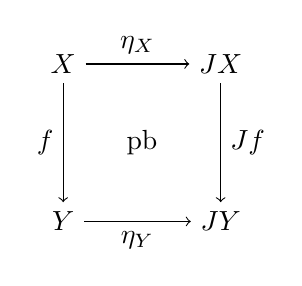
\begin{tikzpicture}
                \node (PB) at (0, 0) {pb};
                \node (X) at (-1, 1) {$X$};
                \node (JX) at (1, 1) {$\mathfrak{J}X$};
                \node (Y) at (-1, -1) {$Y$};
                \node (JY) at (1, -1) {$\mathfrak{J}Y$};
                \draw[->] (X) -- node[above]{$\eta_X$} (JX);
                \draw[->] (Y) -- node[below]{$\eta_Y$} (JY);
                \draw[->] (X) -- node[left]{$f$} (Y);
                \draw[->] (JX) -- node[right]{$\mathfrak{J}f$} (JY);
            \end{tikzpicture}
        \end{gather}
    }

    \newadef{Smooth manifold}{\index{manifold}
        A diffeological space (in its incarnation as a smooth formal set) equipped with a family of local diffeomorphisms from Euclidean spaces (also regarded as formal smooth sets) such that every point of the space lies in the image of at least one such morphism and such that the final topology induced by the plots of the smooth set is paracompact Hausdorff.
    }

    Although we started this section by claiming that we would generalize spaces to the fermionic setting, we have only constructed bosonic spaces. However, everything introduced in this section was formulated in such a way that supergeometry can be included through a minor modification:
    \newdef{Superpoint}{\index{super!point}\index{super!space}
        A space of the form $\text{Spec}(A)$ where $A:=\mathbb{R}\oplus V$ with $V$ a finite-dimensional superalgebra \ref{linalgebra:superalgebra} that forms a nilpotent ideal of $A$. When we take $A$ to be the Grassmann algebra \ref{tensor:exterior_algebra} on $n$ generators we obtain the odd space $\mathbb{R}^{0|n}$. The \textbf{super Euclidean space} $\mathbb{R}^{m|n}$ is obtained as the product of an ordinary Euclidean space $\mathbb{R}^m$ and the superpoint $\mathbb{R}^{0|n}$, i.e. its algebra of smooth functions is $C^\infty(\mathbb{R}^m\times\Pi\mathbb{R}^m)$.
    }
    \newdef{Super smooth set}{\index{smooth!set}
        A sheaf on the category of super Euclidean spaces $\mathbf{SuperCartSp_{diff}}$.
    }

\subsection{Graded manifolds}

    In this section some of the notions from Part \ref{part:diffgeom} will be generalized to the supermanifolds and even general graded manifolds. The general notation $(x^i)$ will be used for the collection of both even and odd coordinates.

    \begin{example}[Supermanifold]\index{super!manifold}
        A super smooth set in the form of a locally ringed space $(M,\mathcal{A})$ that is locally isomorphic to a super Euclidean space, i.e. $\mathcal{A}$ is locally given by $C^\infty(M)\otimes\Lambda^\bullet\mathbb{R}^n$ for some $n\in\mathbb{N}$. More generally, a \textbf{graded manifold} is a locally ringed space that is locally isomorphic to $(\mathbb{R}^m, C^\infty(\mathbb{R}^m)\otimes\text{Sym}(V^*))$ for a graded vector space $V$. (A supermanifold can be recovered by taking $V=\Pi\mathbb{R}^n$.)
    \end{example}

    \begin{theorem}[Batchelor]
        Let $(M,\mathcal{A})$ be an $\mathbb{N}$-graded manifold. There exists a vector bundle $E\rightarrow M$ such that $\mathcal{A}$ is isomorphic to the structure sheaf of $\Gamma(\Lambda^\bullet E)$, i.e. $\mathcal{A}$ is locally given by $\text{Sym}(\Lambda^\bullet E^*)$. If $(M,\mathcal{A})$ is a supermanifold, there exists a vector bundle $E\rightarrow N$ such that $\mathcal{A}$ is locally given by $\Lambda^\bullet E^*$.
    \end{theorem}

    \newdef{Vector fields}{\index{vector field}
        A graded vector field of degree $k$ is a degree-$k$ derivation on $C^\infty(M)$. The integer $k$ is called the \textbf{degree}.
    }
    \newdef{Cohomological vector field}{
        A graded vector field $X$ of degree $1$ that satisfies $[X,X]=0$. Every degree-1 graded vector field satisfies
        \begin{gather}
            [X,X] = 2X\circ X,
        \end{gather}
        which implies that every cohomological vector field defines a coboundary operator on $C^\infty(M)$.

        The de Rham complex $\Omega^\bullet(M)$ is given by $(\Pi TM, Q)$, where $Q$ is the cohomological vector field locally given by
        \begin{gather}
            Q := \sum_{i=1}^ndx^i\partial_i.
        \end{gather}
        Note that the $dx^i$ are here regarded as coordinate functions on $\Pi TM$. The \textbf{degree} of a homogeneous element of $\Omega^\bullet(M)$ is defined as the difference of its graded degree and its form degree.
    }

    \newdef{Poisson manifold}{
        Consider a degree-$k$ symplectic form $\omega$. This form induces a Poisson structure on the algebra $C^\infty(M)$ as follows:
        \begin{gather}
            \{f,g\} := f\overset{\leftarrow}{\partial_i}(\omega^{-1})^{ij}\overset{\rightarrow}{\partial_j}g.
        \end{gather}
        It is not hard to check that this operation is graded-commutative. As in Section \ref{section:hamiltonian_vector_fields}, a Hamiltonian vector field can be defined for any smooth function $H\in C^\infty(M)$:
        \begin{gather}
            \omega(X_H, \cdot) = -dH(\cdot).
        \end{gather}
    }

    \begin{property}[Euler vector field]\index{Cartan!magic formula}\index{Lie!derivative}
        Consider the graded vector field
        \begin{gather}
            E := \sum_{i=1}^n\deg(x^i)x^i\partial_i.
        \end{gather}
        The Lie derivative $\mathcal{L}_E$, defined through the Cartan formula
        \begin{gather}
            \mathcal{L}_E := \iota_Ed + (-1)^{\deg(E)}d\iota_E,
        \end{gather}
        acts on homogeneous forms by multiplication by their degree.
    \end{property}
    \begin{property}
        Every closed differential form of degree $k>0$ is exact. More generally it holds that the de Rham cohomology of a graded manifold is isomorphic to the de Rham cohomology of its body.
    \end{property}
    \begin{result}
        Consider a Hamiltonian cohomological vector field $Q$. There exists a Hamiltonian function $S$ such that
        \begin{gather}
            Qf = \{S,f\}
        \end{gather}
        for all $f\in C^\infty(M)$. If the symplectic form has degree $k$, the function $S$ can be chosen to be of degree $k+1$ and, accordingly, $\{S,S\}$ will be of degree $k+2$. Now, the identity $[Q,Q] = 0$ also implies that $\{S,S\}$ is a constant and since all constants are of degree 0, it follows that
        \begin{gather}
            \label{hdg:classical_master_equation}
            \{S,S\}=0
        \end{gather}
        whenever $k\neq-2$. This equation is often called the \textbf{classical master equation}.

        If $\omega$ if of degree 1, it was shown by \textit{Schwarz} that $(M,\omega)$ is symplectomorphic to $\Pi TM$, such that the Poisson bracket is mapped to the Schouten-Nijenhuis bracket and the Hamiltonian $S$ is mapped to a Poisson bivector field exactly if it satisfies the master equation.
    \end{result}

    \newdef{BV integral}{\index{Batalin-Vilkovisky!integral}\index{gauge}
        Consider a symplectic $m|m$-dimensional supermanifold $(M,\omega)$ where $\omega$ is odd. Let $\psi$, the \textbf{gauge fixing fermion}, be an odd function of half of the coordinates (denote these by $q$). This function determines a projectable Lagrangian submanifold $L_\psi\subset\Pi T^*\mathbb{R}^m$ by the Maslow-H\"ormander theorem \ref{symplectic:maslow_hormander}. The Batalin-Vilkovisky integral of a function $f\in C^\infty(M)$ with respect to $\psi$ is defined as
        \begin{gather}
            \int_{L_\psi}f := \left.\int f\right|_{p_i=\partial_{q^i}\psi}d^mq.
        \end{gather}

        Define the odd (BV) Laplacian as
        \begin{gather}
            \Delta_{\text{BV}} := \sum_{i=1}^m(-1)^{\deg(q^i)}\frac{\partial^2}{\partial q^i\partial p_i}.
        \end{gather}
        This operator satisfies $\Delta_{\text{BV}}f = -\frac{1}{2}\text{div}X_f$ for all $f\in C^\infty(M)$, where $\text{div}$ denotes the divergence \ref{riemann:divergence} with respect to the standard Berezinian volume form. The BV integral and BV Laplacian interact in the following way:
        \begin{enumerate}
            \item If $f=\Delta_{\text{BV}}g$, then $\int_{L_\psi}f = 0$ for all gauge fixing fermions $\psi$ (whenever the BV integral is defined).
            \item If $\Delta_{\text{BV}}f=0$, $\deriv{}{t}\int_{L_{\psi_t}}f=0$, where $\{\psi_t\}_{t\in\mathbb{R}}$ is a continuous family of gauge fixing fermions (whenever the BV integral is defined).
        \end{enumerate}
    }
    \begin{formula}[Quantum master equation]
        Consider the case of a function $f:=e^{i/\hbar S}$ where $S$ is even. Because
        \begin{gather}
            \Delta f = \frac{i}{\hbar}\Delta S e^{i/\hbar S} + \left(\frac{i}{\hbar}\right)^2\frac{1}{2}\{S,S\}e^{i/\hbar S},
        \end{gather}
        the condition that $f$ is harmonic is equivalent to $S$ satisfying
        \begin{gather}
            \frac{1}{2}\{S,S\}-i\hbar\Delta S=0.
        \end{gather}
        This equation is called the quantum master equation. Expanding $S$ as a power series in $\hbar$ shows that the constant term satisfies the classical master equation \ref{hdg:classical_master_equation}.
    \end{formula}

\section{Higher geometry}

    In this section some notions of groups, Lie groups and groupoids (Sections \ref{section:groups}, \ref{section:lie_groups} and \ref{section:groupoids} respectively) are extended the setting of higher category theory.

\subsection{Groups}

    \newdef{Lie groupoid\footnotemark}{\index{Lie!groupoid}\label{hdg:lie_groupoid}
        \footnotetext{In a similar way we could define \textit{topological groupoids, \'etal\'e groupoids}, ...}
        A groupoid internal to $\mathbf{Diff}$.

        Note that Definition \ref{cat:internal_category} requires the existence of pullbacks (of the source and target morphisms). In the category $\mathbf{Diff}$ this is equivalent to assuming that the source and target morphisms are (surjective) submersions.
    }
    \remark{In the Ehresmannian approach one gives the manifold of composable morphisms $D_1\times_{D_0}D_1$ as part of the data. Hence we do not have to assume anything about the source and target morphisms.}

    \newdef{Lie algebroid}{\index{Lie!algebroid}\index{anchor}
        A vector bundle $\pi:E\rightarrow M$ together with a vector bundle morphism $\rho:E\rightarrow TM$, called the \textbf{anchor map}, and a Lie bracket on $\Gamma(E)$ such that the following Leibniz-type property is satisfied:
        \begin{gather}
            [X, fY] = f[X, Y] + \rho(X)(f)Y.
        \end{gather}
        This property also implies that $\rho$ preserves the Lie bracket:
        \begin{gather}
            \rho([X, Y]) = [\rho(X), \rho(Y)].
        \end{gather}
    }
    \begin{example}[Tangent Lie algebroid]\index{pair!groupoid}
        The tangent bundle over a smooth manifold is a Lie algebroid with $\rho\equiv\text{id}$.

        Both the fundamental groupoid $\mathbf{\Pi_1}(M)$ (see definition \ref{topology:fundamental_groupoid}) and the pair groupoid\footnote{The objects are the elements of $M$ and between every two objects there exists exactly one morphism, i.e. $\text{hom}(\mathbf{M\times M})\equiv M\times M$.} $\mathbf{M\times M}$ integrate the tangent Lie algebroid.
    \end{example}

    One can generalize the dual construction of $L_\infty$-algebras \ref{hda:l_infinity_bis} even further:
    \newdef{$L_\infty$-algebroid}{\index{Lie!algebroid}
        Consider the construction of the Chevalley-Eilenberg algebra for a $L_\infty$-algebra. By replacing the base field by a smooth algebra $C^\infty(M)$ for some smooth manifold $M$ and the (graded) vector space $V$ by a module of sections $\Gamma(E)$ of a (graded) vector bundle $E\rightarrow M$, one obtains the notion of a $L_\infty$-algebroid.
    }
    \begin{property}
        $L_\infty$-algebras can be recovered by considering the special case $M=\{\ast\}$.
    \end{property}

    \begin{example}[de Rham complex]
        Consider the tangent algebroid of a smooth manifold $M$. The associated Chevalley-Eilenberg complex
    \end{example}

    \newdef{Weak 2-group}{\index{group!categorical}\index{2!group}
        Let $(\mathbf{C},\otimes,\mathbf{1})$ be a monoidal category. This category is called a weak 2-group, \textbf{categorical group} or \textbf{gr-category} if it satisfies the following conditions:
        \begin{itemize}
            \item All morphisms are invertible.
            \item Every object is weakly invertible with respect to the monoidal structure.
        \end{itemize}
        By property \ref{cat:monoidal_or_2} we can equivalently define a weak 2-group as a 2-category with a single object, weakly invertible 1-morphisms and invertible 2-morphisms.
    }

    \newdef{2-groupoid}{\index{2!groupoid}
        A 2-groupoid is a 2-category in which all 1-morphisms are invertible and every 2-morphisms has a ''vertical'' inverse. (The ''horizontal'' inverse can be constructed from the other ones.)
    }
    \newdef{$\infty$-groupoid}{
        A $\infty$-category in which all morphisms are invertible. This is equivalent to a $(\infty,0)$-category in the language of $(n,r)$-categories.
    }

    \newdef{Strict 2-group}{
        A (strict) 2-group is defined as a (strict) 2-groupoid with only one object. From this it follows that the set of 1-morphisms forms a group and so does the set of 2-morphisms under horizontal composition. However, the 2-morphisms do not form a group under vertical composition\footnote{Because the sources/targets may not match up.}.

        This definition is equivalent to the following internal version: a (strict) 2-group is a group object in $\mathbf{Cat}$ or an internal category in $\mathbf{Grp}$. If we replace $\mathbf{Grp}$ by $\mathbf{Lie}$ we obtain the notion of a (strict) Lie 2-group.
    }

    \begin{property}[Lie crossed modules]\index{module!crossed}\index{differential!crossed module}
        The 2-category of (strict) 2-groups is biequivalent to the 2-category of (Lie) crossed modules \ref{group:crossed_module}. Given a 2-group $\mathcal{G}$, we obtain a crossed module as follows:
        \begin{itemize}
            \item $G:=\text{ob}(\mathcal{G})$,
            \item $H:=\{h\in\text{hom}(\mathcal{G}):\mathfrak{s}(f)=e\}$,
            \item $t(h):=\mathfrak{t}(h)$, and
            \item $\alpha(g)h := \mathbbm{1}_gh\mathbbm{1}_g^{-1}$
        \end{itemize}
        where $\mathfrak{s},\mathfrak{t}$ are the source and target morphisms in $\mathcal{G}$.

        To every Lie crossed module we can also assign a \textbf{differential crossed module}. This consists of the following data:
        \begin{enumerate}
            \item two Lie algebras $\mathfrak{g},\mathfrak{h}$,
            \item a Lie algebra morphism $\partial:\mathfrak{h}\rightarrow\mathfrak{g}$, and
            \item a Lie algebra morphism $\rho:\mathfrak{g}\rightarrow\text{Der}(\mathfrak{h})$.
        \end{enumerate}
        The equivariance and Peiffer conditions induce similar conditions for the above data:
        \begin{itemize}
            \item $\partial(\rho(h)g) = [h,\partial g]$, and
            \item $\rho(\partial h)(h') = [h,h']$
        \end{itemize}
        where $g\in\mathfrak{g}$ and $h,h'\in\mathfrak{h}$. The biequivalence of crossed modules and strict 2-groups induces a biequivalence of differential crossed modules and strict Lie 2-algebras.
    \end{property}

    \begin{example}[Automorphism 2-group]
        Given a Lie group $H$, we can construct a crossed module with $G:=\text{Aut}(H)$, $t$ assigning inner automorphisms (conjugations) and $\alpha$ the obvious map. The associated 2-group $\text{AUT}(H)$ gives a 2-group of symmetries of $H$, i.e. it is the automorphism 2-group of $H$ in the 2-category $\mathbf{Lie}$.
    \end{example}

    \newdef{Exponentiable groups}{\index{exponentiable}
        Smooth groups for which every smooth function $f:[0,1]\rightarrow\mathfrak{g}$ corresponds to a smooth function $g:[0,1]\rightarrow G$ such that
        \begin{gather}
            \deriv{}{t}g(t) = f(t)g(t)
        \end{gather}
        with $g(0) = e$, are said to be exponentiable. A smooth 2-group is said to be exponentiable if both of its component groups are exponentiable. Since all Lie groups are exponentiable, all Lie 2-groups are also exponentiable
    }

    \begin{remark}[Lie's third theorem]\index{Lie!third theorem}
        In ordinary Lie theory Lie's third theorem states that every (finite-dimensional) Lie algebra can be obtained as the infinitesimal version of a Lie group. However, this does not carry over to the 2-group setting. Consider for example the Lie 2-algebras $\mathfrak{g}_\lambda$ constructed in example \ref{hda:gk_lie_2_algebra}. As shown in \cite{HDA5} only $\mathfrak{g}_0$ gives rise to a Lie 2-group (or even a topological 2-group).
    \end{remark}

\subsection{Spaces}

    \newdef{Smooth 2-space}{
        To overcome the problem encountered in definition \ref{hdg:lie_groupoid} above, we should pass from $\mathbf{Diff}$ to $\mathbf{C^\infty}$. It can be shown that this category admits all pullbacks, quotients, path spaces, etc. As such we define a smooth 2-space as a category internal to $\mathbf{C^\infty}$.

        In the remainder of this chapter we will assume all spaces to be smooth in the general sense. The notions of 2-groups as introduced in the previous section are easily generalized to this wider setting.
    }

    \newdef{2-group action}{\index{group!action}
        Consider a smooth 2-group $\mathcal{G}$ and a smooth 2-space $E$. A strict action of $\mathcal{G}$ on $E$ is a smooth homomorphism $\mathcal{G}\rightarrow\text{AUT}(E)$, i.e. a smooth map preserving products and inverses.
    }

    \newdef{Thin homotopy}{\index{homotopy!thin}
        Let $M$ be a smooth manifold. A smooth homotopy $H:[0,1]^2\rightarrow M$ is said to be thin if
        \begin{gather}
            H(s, t) = F(s)
        \end{gather}
        for some smooth $F$ near $t=0,1$ and if it pulls back\footnote{See section \ref{section:forms}.} every two-form to 0:
        \begin{gather}
            \forall \omega\in\Omega^2(M): H^*\omega = 0.
        \end{gather}
    }
    \newdef{Lazy path\footnotemark}{\index{path!lazy}\index{sitting instants}
        \footnotetext{Also called a path with \textbf{sitting instants}.}
        Let $M$ be a smooth manifold. A path $f:[0,1]\rightarrow M$ is said to be lazy if it is locally constant on some neighbourhoods of $0$ and $1$.
    }

    \newdef{Path groupoid}{\index{groupoid!path}\label{hdg:path_groupoid}
        Let $M$ be a smooth space. The path groupoid $\mathcal{P}_1(M)$ is the groupoid (in fact a smooth groupoid and hence a smooth 2-group) which has the points of $M$ as objects and the thin homotopy classes of lazy paths with fixed endpoints on $M$ as morphisms.\footnote{The laziness combined with the first condition of thin homotopies implies that the morphisms of the groupoid are (locally) constant near the full boundary of their domain.}

        In fact by suitably generalizing the smoothness properties of the homotopies and paths, we can ''easily'' extend this definition to surface, volumes and so on. This results in the $n$-path $n$-groupoid $\mathcal{P}_n(M)$.
    }
    \sremark{The restriction to lazy paths is required to ensure the smoothness of composite paths. The quotient by thin homotopies is required to ensure the validity of the associativity and invertibility properties.}

    ?? COMPLETE ??

\section{2-Bundles}

    A first step is the generalization of the categorical definition of a bundle \ref{diff:bundle}, i.e. as an object of a slice category:
    \newdef{2-bundle}{\index{bundle}
        A smooth 2-bundle is a triple $(E,B,\pi)$ where both $E$ and $B$ are smooth 2-spaces and $\pi$ is a smooth map.
    }
    \newdef{Locally trivial 2-bundle}{
        For a smooth 2-space we define a locally trivial 2-bundle with typical fibre $F$ as a 2-bundle $(E,B,\pi)$ with an open cover $\{U_i\}_{i\in I}$ of $B$ such that for every $i\in I$ there exists an equivalence $\varphi_i:E|_{U_i}\cong U_i\times F$ that makes the diagram below commute.

        \begin{figure}[ht!]
            \centering
            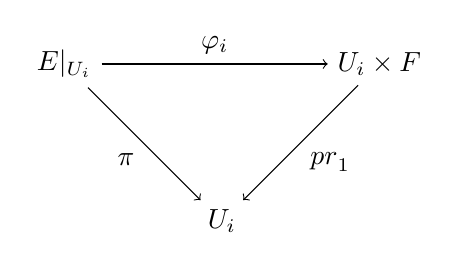
\begin{tikzpicture}
                \node (E) at (-2, 0) {$E|_{U_i}$};
                \node (UF) at (2, 0) {$U_i\times F$};
                \node (U) at (0, -2) {$U_i$};
                \draw[->] (E) -- node[above]{$\varphi_i$} (UF);
                \draw[->] (E) -- node[below left]{$\pi$} (U);
                \draw[->] (UF) -- node[below right]{$\text{pr}_1$} (U);
            \end{tikzpicture}
        \end{figure}
        We should note that the existence of such a cover is not a trivial matter. The general definition becomes quite involved when allowing for arbitrary smooth 2-spaces $B$. For convenience we will always assume that $B$ is an ordinary smooth space regarded as a 2-space with only trivial morphisms.

        As was the case in definition \ref{diff:fibre_bundle}, we can also characterize locally trivial 2-bundles by their transition data. Since the trivilizations $\varphi_i$ are equivalences, they admit an inverse (up to an invertible 2-map) and we can thus construct transition maps $\varphi_i\varphi_j^{-1}=U_{ij}\times F\cong U_{ij}\times F$ as usual. By the commutative diagram above, these transition maps only act on the fibre $F$. Because $\varphi_i\varphi_j^{-1}$ is itself an (auto)equivalence, the action on $F$ is given by a functor $g_{ij}:U_{ij}\rightarrow\text{AUT}(F)$ where the 2-space $\text{AUT}(F)$ is the \textit{coherent }2-\textit{group}\footnote{Instead of the strict invertibility of maps in our definition of 2-groups, we should allow them to be invertible up to 2-isomorphisms which themselves satisfy certain coherence conditions.} of autoequivalences of $F$ together with invertible 2-maps between them.

        The interesting (and important) part is how the cocycle conditions \ref{diff:G_cocycle_condition} and \ref{diff:G_cocycle_conditions} for the maps $g_{ij}$ are modified. Since the equivalences $g_{ij}$ are only invertible up to 2-maps, we cannot expect these conditions to hold as equations. Instead we obtain 2 higher transition maps (i.e. natural isomoprhisms) $h_{ijk}:g_{ij}\circ g_{jk}\Rightarrow g_{ik}$ and $k_i:g_{ii}\Rightarrow\text{id}$. These higher data should in turn satisfy the necessary conditions coming from associativity and unitality constraints (similar to the coherence conditions in section \ref{section:hda_group_cohomology}).
    }
    \newdef{$\mathcal{G}$-bundle}{\index{principal!bundle}
        A locally trivial 2-bundle with typical fibre $F$ is said to have the 2-group $\mathcal{G}$ as its structure (2-)group if the transition data factor through an action $\mathcal{G}\rightarrow\text{AUT}(F)$. If $F=\mathcal{G}$, we call the 2-bundle a \textbf{principal $\mathcal{G}$-2-bundle}.
    }
    \begin{remark}[Gerbes]\index{gerbe}
        If we choose the transition maps $k_i$ to be trivial and let $\mathcal{G}$ be respectively the trivial Lie 2-group associated to an Abelian Lie group $G$ or the automorphism 2-group of a Lie group $H$, we obtain Abelian and non-Abelian \textit{gerbes}. In fact it can be shown that the 2-category of principal $2$-bundles is equivalent to the 2-category of gerbes for every Lie 2-group of the aforementioned type.
    \end{remark}

    By categorifying definition \ref{diff:holonomy_functor} of principal connections we can define connections for principal $n$-bundles:
    \newdef{$n$-connection}{\index{connection!principal}
        Let $M$ be a smooth space and let $G$ be a Lie $n$-groupoid. Given a locally trivial principal $n$-bundle $P$ over $M$ we define an $n$-connection with $n$-holonomy through the following data:
        \begin{enumerate}
            \item for every coordinate chart $U_i\subset M$ a local holonomy $n$-functor
            \begin{gather}
                \text{hol}_i:\mathcal{P}_n(U_i)\rightarrow G;
            \end{gather}
            \item for every double intersection $U_{ij}$ a 1-transfor (i.e. an $n$-natural transformation)
            \begin{gather}
                g_{ij}:\text{hol}_i\Rightarrow\text{hol}_j;
            \end{gather}
            \item for every triple intersection $U_{ijk}$ a 2-transfor
            \begin{gather}
                f_{ijk}:g_{ij}\circ g_{jk}\Rrightarrow g_{ik};
            \end{gather}
            \item and so on...
        \end{enumerate}
        This is equivalently given by a global $n$-functor
        \begin{gather}
            \text{hol}:\mathcal{P}_n(M)\rightarrow\mathbf{Trans}_n(P).
        \end{gather}
    }

    ?? ADD GERBES (e.g. BRYLINSKI) AND PERHAPS DELIGNE COHOMOLOGY ??

\section{Space and quantity}

    In this section we move our focus back from (differential) geometry to the general notion of what spaces and observables are. From the start we will assume that we are working in an enriched setting where $\mathcal{V}$ is a cosmos \ref{cat:cosmos}. The categories $\mathbf{C}$ of interest will be assumed to be small and $\mathcal{V}$-enriched.

    In the previous sections we defined spaces modelled on a base space $X$, or more generally on a category of spaces $\mathbf{S}$, as sheaf or even a concrete sheaf on a suitable site. Here we relax this notion as much as possible:
    \newdef{Space}{\index{space}
        A (generalized) space modelled on a category $\mathbf{C}$ is a presheaf on $\mathbf{C}$.

        As before we can interpret the object $X(C)$ as the collection of ''probes'' from $C$ to $X$. The Yoneda lemma and embedding assure that ordinary test spaces in $\mathbf{C}$ can be viewed as spaces modelled on $\mathbf{C}$ and that their probes are indeed the ordinary maps in $\mathbf{C}$.
    }
    In a similar vein we can define observables as maps out of a space:
    \newdef{Quantity}{\index{quantity}
        A (generalized\footnote{It is generalized because it is ''measured'' on category instead of on a single object.}) quantity on a category $\mathbf{C}$ is a copresheaf on $\mathbf{C}$.
    }

    \begin{property}[Isbell duality]\index{Isbell duality}
        Given a space $X$ we can look at the quantities that live on it (in ordinary geometry this would have been its algebra of functions). This defines a functor:
        \begin{gather}
            \mathcal{O}:\mathbf{Psh(C)}\rightarrow\mathbf{coPsh}^{op}(\mathbf{C}):X\mapsto\hom_{\mathbf{Psh(C)}}(X, \mathcal{Y}-).
        \end{gather}
        Similarly, given a quantity $Q$ we can ask on which space it behaves as the algebra of functions. This also defines as functor:
        \begin{gather}
            \text{Spec}:\mathbf{coPsh}^{op}(\mathbf{C})\rightarrow\mathbf{Psh(C)}:Q\mapsto\hom_{\mathbf{coPsh(C)}}(\mathcal{Y}^{op}-, Q)
        \end{gather}
        where $\mathcal{Y}^{op}$ denotes the co-Yoneda embedding $\mathbf{C}\rightarrow\funccat{C}{\mathcal{V}}^{op}:c\mapsto\mathbf{C}(, -)$.

        The incredible result is now that $(\mathcal{O}\dashv\text{Spec})$ is an adjunction (suitably called the \textbf{Isbell adjunction}). Objects that are preserved (up to isomorphism) under the associated (co)monad are said to be \textbf{Isbell self-dual}.
    \end{property}
    \begin{example}[Cartesian spaces]
        When working over the site $\mathbf{CartSp}$ (with its usual topology) and restrict to coherent sheaves and product-preserving presheaves, the Isbell adjunction maps spaces to smooth algebras.
    \end{example}